\documentclass[11pt]{article}

\usepackage{arxiv}
\usepackage[utf8]{inputenc}
\usepackage[T1]{fontenc}
\usepackage{lmodern}
\usepackage{microtype}
\usepackage{hyperref}
\usepackage{url}
\usepackage{booktabs}
\usepackage{amsfonts}
\usepackage{amsmath}
\usepackage{amssymb}
\usepackage{nicefrac}
\usepackage{graphicx}
\usepackage{xcolor}
\usepackage{multirow}
\usepackage{subcaption}
\usepackage{enumitem}
\usepackage{cleveref}
\usepackage[numbers,sort&compress]{natbib}
\usepackage{tikz}
\usetikzlibrary{positioning,arrows.meta,shapes.geometric,fit,calc}
\usepackage{pgfplots}
\pgfplotsset{compat=1.18}

\hypersetup{
  colorlinks=true,
  linkcolor=blue!50!black,
  citecolor=blue!50!black,
  urlcolor=blue!50!black,
}

\title{Format Matters More Than Capacity:\texorpdfstring{\\}{ }Distilling Multimodal Interaction Scaling into 8B Models}

\author{
  Bojie Li\\
  Pine AI \\
  \texttt{boj@19pine.ai}
}

\runningtitle{Format Matters More Than Capacity}

\date{}

\begin{document}

\maketitle

\begin{abstract}
\emph{Interaction scaling} --- the SOTA pattern of iteratively writing, rendering, critiquing, and revising an artifact --- is the dominant test-time scaling regime for multimodal generation tasks. Deploying it depends on a costly large model in the loop. We ask whether interaction scaling can be \emph{distilled} into an 8B-class student.
We find a sharp asymmetry: in a \emph{compressed-trajectory markdown} format, where the student emits critique-and-revise blocks and an external scaffold handles I/O, an 8B Qwen3-VL student reaches 44\% pass@1 and 56\% pass@3 on hard held-out tasks --- 0.51$\times$ the teacher's capability single-shot, climbing to 0.70$\times$ at pass@2 on truly novel tasks. In a \emph{fully agentic tool-use} format, where the same student must orchestrate \texttt{write\_file}/\texttt{read\_file}/\texttt{bash} calls itself, the same recipe collapses to 6\% pass@1 (22\% pass@3), with webpages stuck at 0/5 \emph{across every configuration we tested} (8B/30B-A3B/32B; bf16/4-bit/8-bit; 18 to 51 SFT examples; verbose vs.\ compact teacher; 0/44 on out-of-distribution tasks). A joint statistical test puts the true webpage-keep rate under the agentic format below 11.3\% with 95\% confidence.
A 4$\times$ capacity scaling closes only a small fraction of the gap (8B$\to$32B raises judge-keep from 1/18 to 3/18); a 2$\times$2 base-vs-SFT ablation shows that markdown SFT lifts the base by +2 keeps while agentic SFT \emph{regresses} the base by $-1$. A cross-format eval (each adapter run at both deployments) is decisive: every adapter --- including the agentic-trained v8 --- does better at markdown deployment than at agentic deployment, and the agentic-trained adapter is 5$\times$ better at markdown deployment (5/18) than at its own native deployment (1/18). The format gap is therefore primarily a \emph{deployment-time mechanics} effect; SFT can imprint format but cannot rescue the agentic format from its structural disadvantage at this scale.
We additionally surface three counterintuitive recipe findings: (a) a U-curve in retained teacher reasoning length, with the optimum at the \emph{student's} coherence horizon (not the teacher's); (b) more SFT data \emph{regresses} judge-keep across three independent confirmations; and (c) expert-iteration RFT polishes consistency but kills pass@k inference scaling ($-17$pp pass@3) --- the model's variance \emph{is} the inference-scaling lever.
The operational implication for deploying interaction scaling at 8B scale is unambiguous: external scaffolding over a markdown-emitting student dominates a tool-using agentic student by an order of magnitude in cost-per-success, and is robust to the choice of how the student was fine-tuned.
\end{abstract}

\section{Introduction}
\label{sec:intro}

State-of-the-art multimodal generation (web pages, slides, technical figures, video, code-with-tests) increasingly relies on \emph{interaction scaling} at test time: the model writes an initial artifact, renders or executes it, reads the result, identifies defects, and revises. This loop --- variants of which appear under names including ReAct, Voyager, Reflexion, and self-refine --- routinely yields large gains over single-shot inference, but it depends on a strong, often expensive model held in the loop.

Two practical questions follow:
\begin{enumerate}[leftmargin=*]
  \item \textbf{Can the interaction loop be distilled into a small student} so that the loop runs cheaply at deployment?
  \item \textbf{What format should the distilled student emit}? In particular, should the student call tools itself (\emph{agentic format}) or should an external scaffold do file I/O and rendering while the student emits only critique-and-revise blocks (\emph{markdown format})?
\end{enumerate}

We give an empirical answer in both directions.

\paragraph{Markdown distills well.} An 8B Qwen3-VL student, trained on $\sim$37 judge-filtered teacher trajectories with reasoning capped at the \emph{student's} coherence horizon ($\sim$1500 chars), reaches 44\% judge-keep at pass@1 and 56\% at pass@3 on a suite of 18 hard held-out tasks (5 code, 5 webpages, 8 slides) --- starting from 0\% baseline by the same judge. The student transfers 0.51$\times$ of the 235B teacher's single-shot capability and 0.70$\times$ at pass@2 on 44 truly novel tasks.

\paragraph{Agentic does not.} The \emph{same} pipeline, replacing markdown emission with three general tools (\texttt{write\_file}, \texttt{read\_file}, \texttt{bash}) and a per-trajectory sandbox, yields 6\% pass@1 / 22\% pass@3. We ablate this negative result across five orthogonal axes --- model capacity ($8\mathrm{B} \to 30\mathrm{B\text{-}A3B} \to 32\mathrm{B}$), precision (bf16 / 8-bit / 4-bit), SFT data scale (18 / 31 / 51 examples), teacher style (verbose / compact), and inference sampling (pass@1, pass@2, pass@3) --- and find that \emph{webpage judge-keep is 0/5 in every configuration}. Capacity helps modestly on code (1/5 $\to$ 3/5) but not on visual tasks. The format thus has a structural quality floor for visual generation in the 8B--30B regime.

\paragraph{Three counterintuitive recipe findings} emerged from the markdown sweep that we believe will recur in similar distillation work:
\begin{enumerate}[leftmargin=*,topsep=0.2ex,itemsep=0.2ex]
  \item \textbf{U-curve in reasoning retention.} Stripping the teacher's reasoning collapses the student to format-imitating identical-retry. Retaining all of it overflows the student's coherence horizon. The optimum is the \emph{student's} typical reasoning length, not the teacher's.
  \item \textbf{More SFT data regresses.} Three independent attempts to scale the SFT corpus past 37 examples (V5: 50, V6: 57, RFT: 61) each lost ground. Quality dominates quantity; the student cannot bootstrap above its current capability via judge-filtered self-play.
  \item \textbf{RFT (expert iteration) is anti-pass@k.} Rejection-sampling-based fine-tuning improved every per-turn consistency metric (identical-retry, no-artifact, addresses-review) but \emph{lost} 17pp at pass@3. The model's variance --- punishable as inconsistency --- \emph{is} the inference-scaling budget. For deployment with sampling, do not post-train past SFT.
\end{enumerate}

\paragraph{Contributions.}
\begin{itemize}[leftmargin=*,topsep=0.2ex,itemsep=0.2ex]
  \item A reproducible recipe for distilling multimodal interaction-scaling behavior into an 8B model that retains a meaningful fraction of the 235B teacher's capability (\Cref{sec:markdown}).
  \item An exhaustive five-axis negative result for the agentic tool-use variant of the same pipeline (\Cref{sec:agentic}) --- corroborated by a 2$\times$2 base-vs-SFT ablation, a Bonferroni-style joint test on the webpage 0-floor, an out-of-distribution generalization test (0/44), and inter-judge agreement on a second judge.
  \item A cross-format eval (\Cref{sec:crossformat}) showing that the format gap is primarily at deployment time, not in SFT data: every adapter does better at markdown deployment than at agentic deployment, and the agentic-trained adapter is 5$\times$ better at markdown deployment than at its native deployment.
  \item Three counterintuitive empirical findings about distillation hyperparameters and post-SFT polishing, validated across multiple seeds and a separate generalization set (\Cref{sec:markdown,sec:discussion}).
  \item An operational recommendation: at 8B scale, deploy interaction scaling via an external scaffold over a markdown-emitting student. The scaffold is 10$\times$ cheaper per kept task than any agentic configuration we tested, and is robust to whether the student was fine-tuned on markdown traces or agentic traces.
\end{itemize}

\section{Related Work}
\label{sec:related}

\paragraph{Test-time scaling.} A growing body of work shows that allocating extra compute at inference --- via chain-of-thought \citep{wei2022chain}, self-consistency \citep{wang2023selfconsistency}, tree search \citep{yao2023tree}, iterative refinement \citep{shinn2023reflexion,madaan2023selfrefine}, or compute-optimal allocation \citep{snell2024scaling,beeching2024searchscale} --- improves task performance well past single-shot ceilings. The most recent reasoning-trained systems (DeepSeek-R1, Kimi K1.5; \citealp{deepseek2025r1,kimi2025k15}) demonstrate that test-time-scaled behavior can be elicited via large-scale RL on a strong base. Our \emph{interaction-scaling} regime is a specialization of iterative refinement in which the refinement signal is grounded in tool execution (test runs, headless browser renders) rather than in self-evaluation alone, and our distillation question targets the much smaller (8B-class) student regime.

\paragraph{Agentic LLMs and multimodal benchmarks.} Tool-augmented LLMs \citep{schick2023toolformer,patil2024gorilla} and agentic frameworks that interleave reasoning and acting \citep{yao2023react,wang2023voyager} have become the dominant deployment paradigm for tasks that require external feedback. The natural evaluation environment for such systems --- agents that operate computers, browse the web, or render artifacts --- is captured in benchmarks like OSWorld \citep{xie2024osworld} and VisualWebArena \citep{koh2024visualwebarena}. Most evaluations of these systems use frontier models in the loop; the cost of replicating them at deployment motivates our distillation question.

\paragraph{Distillation of reasoning and tool use.} A separate line distills test-time-scaled behavior of large models into smaller students \citep{magister2023teaching,ho2023largelm,fu2023specializing} or distills tool-using policies \citep{schick2023toolformer,patil2024gorilla}. The recent open-weight reasoning systems --- DeepSeek-R1's distilled checkpoints \citep{deepseek2025r1} and the Kimi K1.5 line \citep{kimi2025k15} --- demonstrate that high-quality test-time-scaled traces \emph{can} distill into smaller students at scale. Most of this work targets text-only tasks and does not isolate the format question we focus on. The closest contemporaneous works distill specific agentic behaviors but do not, to our knowledge, contrast a tool-using student against a markdown-emitting student under matched compute and data budgets.

\paragraph{Sampling-based inference scaling and consistency-vs-diversity.} Best-of-$n$ and pass@k inference \citep{chen2021evaluating,brown2024large} rely on output diversity. A long line of work documents that fine-tuning, and especially RLHF \citep{stiennon2020learning,casper2023open}, can collapse this diversity along multiple axes \citep{kirk2024diversity,padmakumar2024writing}. Our finding that rejection-sampling fine-tuning loses 17pp at pass@3 while improving every per-turn consistency metric is a multimodal, multi-turn instance of this same tension --- and provides an actionable deployment recommendation: stop after the first round of careful SFT if pass@k is part of the inference budget.

\section{Experimental Setup}
\label{sec:setup}

\subsection{Tasks and benchmark}

We evaluate on a held-out suite of 18 \emph{hard} tasks across three categories where interaction scaling is known to help: code bug-fixes (5), single-file landing-page web designs (5), and information-dense 1920$\times$1080 slides (8). Each task carries a natural-language description plus, for the visual categories, a list of explicit requirements (e.g., ``hero section with gradient background \texttt{\#1a1a4e}$\to$\texttt{\#6b21a8}, two CTA buttons side by side''). The held-out set was constructed by retaining tasks the 235B teacher \emph{itself} failed on at single-shot under the same judge --- giving a clean ``distillation lift'' baseline. We additionally use 44 newly generated tasks (held-out by construction) to test out-of-distribution generalization.

\subsection{Teacher, students, and judge}

\textbf{Teacher.} Qwen3-VL-235B-A22B (Thinking variant for the markdown setup; Instruct variant for the agentic setup, where the Thinking model emitted malformed JSON tool arguments).

\textbf{Students.} Primary student is Qwen3-VL-8B-Instruct with QLoRA fine-tuning ($r{=}16$, $\alpha{=}32$, dropout 0.05) on attention $+$ MLP modules of the language layers; vision tower frozen. For the agentic ablations we additionally train Qwen3-VL-30B-A3B-Instruct (MoE, 8-bit base via \texttt{bitsandbytes}) and Qwen3-VL-32B-Instruct (4-bit NF4 base, double-quantized).

\textbf{Judge.} Gemini 3 Flash Preview multimodal. The judge sees a structured trace summary (one message per assistant turn), the explicit task spec, and --- for visual tasks --- the actual rendered final screenshot, so that the ``the page looks good'' claim is checked against pixels rather than against the student's own description. The judge returns four binary fields: \texttt{review\_specific}, \texttt{revision\_addresses\_review}, \texttt{final\_meets\_spec}, and a derived \texttt{keep} = AND of the three. For code, \texttt{final\_meets\_spec} is overridden by the deterministic test-suite outcome.

\subsection{Metrics}

We report \texttt{judge-keep} as the primary outcome, since it captures both interaction-quality (the first two judge fields) and final-artifact quality (the third). We complement it with \emph{single-step overflow rate} (the model wrote a tool-call body that exceeded the inference token budget) and \texttt{status=final emitted} (the model declared completion via \texttt{<final>OK</final>}). For pass@k we union judge-kept tasks across $k$ independent samples (different seeds; sampling at $T{=}0.7$, $\mathrm{rep\_penalty}{=}1.0$).

\paragraph{Inter-judge agreement.} To check that the headline gap is not a Gemini-judge artifact, we re-judged two trace sets (V3+fc4k seed1 markdown, and v8 seed42 agentic) using a second judge (Claude Sonnet 4.5, same prompt, same images). Per-task agreement is 86\% (Cohen's $\kappa = 0.55$, moderate). Notably, the two judges agree perfectly on the 18 agentic v8 traces (1/18 keep under both), while Claude is consistently stricter on visual artifacts in the markdown set: V3+fc4k re-scores at 8/18 (Gemini) vs.\ 3/18 (Claude). The directional gap (markdown $\gg$ agentic) holds under either judge, with the under-Claude gap being 3/18 vs.\ 1/18 instead of 8/18 vs.\ 1/18. We retain Gemini as the primary judge throughout for consistency with prior work in the line, and treat Claude's stricter scoring as a sensitivity check.

\subsection{Two formats compared}

\textbf{Markdown format (Phase 5).} The student receives the task spec plus a per-category system prompt that mixes generation and critique-and-revise instructions. Each assistant turn is a single block of markdown: a short \texttt{<think>} reasoning block, an optional critique paragraph, and the artifact in a fenced code block (\texttt{```python}, \texttt{```html}, \ldots). An external harness extracts the artifact, runs the tests / renders the page, and feeds the result (text execution output or rendered PNG) back as the next user message.

\textbf{Agentic format (Phase 6).} The student receives a stripped system prompt and three tool schemas (\texttt{write\_file(path,content)}, \texttt{read\_file(path)}, \texttt{bash(command)}). The student emits OpenAI-style \texttt{<tool\_call>\{json\}</tool\_call>} blocks. A per-trajectory sandbox dispatches each call. Visual feedback flows back as image content in a \texttt{tool} role message (the Qwen3-VL chat template renders this correctly). The student must orchestrate write$\to$render$\to$read$\to$critique cycles itself.

The two formats use the same teacher, the same task suite, the same judge, and matched LoRA hyperparameters and SFT compute. The only differences are: (i) the system prompt, (ii) whether tool calls are emitted by the student or handled by the harness, and (iii) the resulting trace structure used for SFT. \Cref{fig:formats} contrasts a single iteration of the loop in each format.

\begin{figure}[t]
\centering
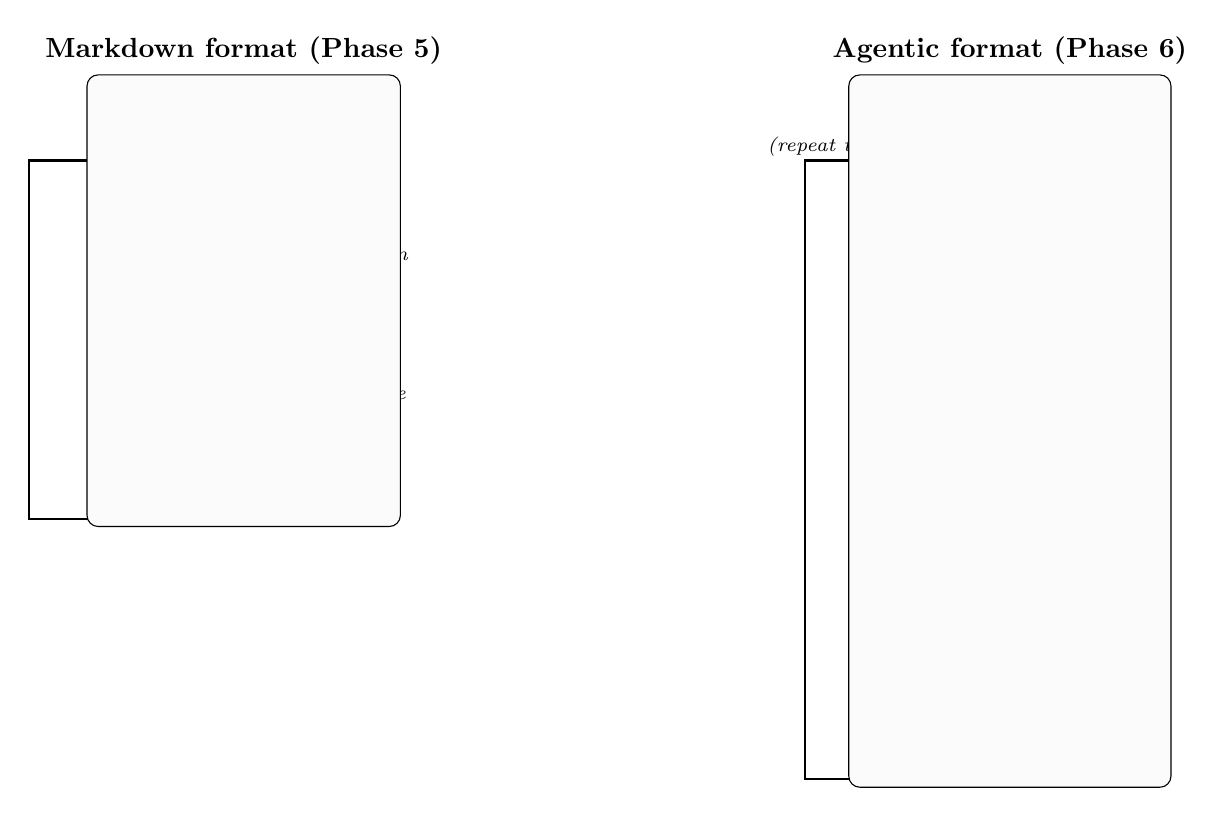
\begin{tikzpicture}[
  node distance=4mm and 5mm,
  font=\footnotesize,
  every node/.style={align=center},
  box/.style={draw, rounded corners=2pt, minimum height=6mm, minimum width=24mm,
              inner sep=2pt, fill=blue!5},
  envbox/.style={draw, rounded corners=2pt, minimum height=6mm, minimum width=24mm,
                 inner sep=2pt, fill=orange!10},
  panel/.style={draw, rounded corners=4pt, inner sep=4mm, fill=gray!3},
  arrow/.style={-{Latex[length=2mm]}, thick},
  payload/.style={font=\scriptsize\itshape, fill=white, inner sep=1pt},
]
% ===== LEFT: markdown =====
\node[box] (m1) {Student emits\\\texttt{<think>}\,plan\,\texttt{</think>}\\\texttt{```html} artifact \texttt{```}\\\texttt{<final>OK</final>}?};
\node[envbox, below=10mm of m1] (m2) {External harness\\extracts artifact,\\renders / runs tests};
\node[envbox, below=of m2] (m3) {Returns rendered PNG\\(or test stdout/err)\\as next user message};

\draw[arrow] (m1) -- node[payload, right=1mm]{markdown turn} (m2);
\draw[arrow] (m2) -- node[payload, right=1mm]{rendered image} (m3);
\draw[arrow] (m3.south) -- ++(0,-3mm) -| ([xshift=-12mm]m1.west) -- (m1.west);

\node[fit=(m1)(m2)(m3), panel, label={[font=\bfseries]above:Markdown format (Phase 5)}] (mp) {};

% ===== RIGHT: agentic =====
\node[box, right=68mm of m1.east, anchor=west] (a1) {Student emits\\\texttt{<tool\_call>}\\\texttt{\{write\_file: ...\}}\\\texttt{</tool\_call>}};
\node[envbox, below=4mm of a1] (a2) {Sandbox writes file\\returns ack};
\node[box, below=4mm of a2] (a3) {Student emits\\\texttt{<tool\_call>}\\\texttt{\{bash: chromium ...\}}\\\texttt{</tool\_call>}};
\node[envbox, below=4mm of a3] (a4) {Sandbox runs bash\\returns exit code};
\node[box, below=4mm of a4] (a5) {Student emits\\\texttt{<tool\_call>}\\\texttt{\{read\_file: out.png\}}\\\texttt{</tool\_call>}};
\node[envbox, below=4mm of a5] (a6) {Sandbox returns image\\(via tool-role msg)};

\draw[arrow] (a1) -- (a2);
\draw[arrow] (a2) -- (a3);
\draw[arrow] (a3) -- (a4);
\draw[arrow] (a4) -- (a5);
\draw[arrow] (a5) -- (a6);
\draw[arrow] (a6.south) -- ++(0,-3mm) -| ([xshift=-12mm]a1.west) -- (a1.west)
  node[payload, midway, above]{(repeat to revise)};

\node[fit=(a1)(a2)(a3)(a4)(a5)(a6), panel,
      label={[font=\bfseries]above:Agentic format (Phase 6)}] (ap) {};
\end{tikzpicture}
\caption{One iteration of the review loop in each format. Blue = student-emitted tokens (counted in the SFT signal); orange = external environment returns. The markdown format compresses the artifact-emit step into one assistant turn that the harness can directly parse and render. The agentic format requires the student to emit three separate tool calls --- inflating the per-turn token cost and adding tool-grammar / sequencing / termination as additional concepts the SFT must internalize.}
\label{fig:formats}
\end{figure}

\section{Markdown Distillation Works}
\label{sec:markdown}

\subsection{Recipe}

Teacher trajectories are collected by running the 235B model in the markdown loop for up to five turns per task. The judge filters trajectories to those satisfying all three of \texttt{review\_specific}, \texttt{revision\_addresses\_review}, and \texttt{final\_meets\_spec}. The 235B teacher's loop produces $\sim$50 raw trajectories on the seed task set; 37 survive the judge.

Each surviving trajectory is converted to a multi-turn SFT example. The teacher's chain-of-thought \texttt{<think>} block is retained but truncated per-turn at a configurable cap; the visual feedback is converted to a downscaled screenshot ($\le$1280px on the long side) embedded in the user turn; the loss is masked to assistant tokens only.

At inference, we apply a \emph{force-close-thinking} logit override that injects \texttt{</think>} after a configurable number of generated tokens if the student has not closed the think block voluntarily, then proceeds with the rest of the response. This bounds the worst-case decode wall-time per turn.

\subsection{Reasoning U-curve and the student's coherence horizon}

\Cref{tab:reasoning-ucurve} sweeps the per-turn reasoning cap. Both shorter (1000) and longer (3000) caps regress relative to 1500. The intuition is mechanical: stripping reasoning collapses the student to format-imitating identical-retry (the Phase 2 failure mode); retaining the full teacher reasoning ($\sim$3K chars median, $\sim$80K max) overruns the student's coherence horizon and produces in-distribution noise.

\begin{table}[t]
\centering
\caption{Reasoning-cap U-curve. SFT recipe sweep on Qwen3-VL-8B-Instruct (37 judge-kept teacher traces; same inference protocol). Identical-retry counts repeated emission of byte-identical artifacts across turns.}
\label{tab:reasoning-ucurve}
\begin{tabular}{lcccc}
\toprule
Variant & Reasoning cap (chars) & Judge-keep & Identical-retry & no-artifact \\
\midrule
V1 (no reasoning) & 0 & 6\% & 67\% & 2 \\
V4 & 1000 & 11\% & 35\% & 9 \\
V2 & 3000 & 17\% & 32\% & 8 \\
\textbf{V3 (chosen)} & \textbf{1500} & \textbf{44\%} & \textbf{10\%} & 6 \\
\bottomrule
\end{tabular}
\end{table}

We frame this as the \emph{student's coherence horizon}: the longest reasoning span the 8B model can both reproduce in training and faithfully complete at inference. Train at the student's horizon, not the teacher's.

\subsection{Force-close-thinking is a free wall-time win}

\Cref{tab:fc-sweet-spot} sweeps the inference-time force-close threshold. Force-closing too aggressively (2000 tokens) costs 16pp judge-keep; force-closing at 4000 tokens matches V3's quality with a 2.2$\times$ wall-time speedup.

\begin{table}[t]
\centering
\caption{Force-close-think inference sweep (V3 SFT, identical decode otherwise).}
\label{tab:fc-sweet-spot}
\begin{tabular}{lcc}
\toprule
Variant & Judge-keep & Avg seconds/task \\
\midrule
V3 baseline (no fc) & 44\% & 501 \\
V3 + fc=2000 & 28\% & 202 \\
\textbf{V3 + fc=4000 (chosen)} & \textbf{44\%} & \textbf{225} \\
\bottomrule
\end{tabular}
\end{table}

\subsection{Quality dominates quantity}

We made three independent attempts to enlarge the SFT corpus past V3's 37 examples (\Cref{tab:data-scale}). Each regressed the headline metric. V5 added 13 judge-rejected traces from the same teacher; V6 added 20 judge-kept traces from a weaker (30B) teacher; RFT collected 61 judge-kept self-rolled trajectories from V3 itself. None lifted judge-keep above the 8/18 ceiling, and the most ``polished'' (RFT) carried a hidden cost we describe below.

\begin{table}[t]
\centering
\caption{Three SFT data-scale attempts past V3's 37 examples. All regressed.}
\label{tab:data-scale}
\begin{tabular}{lccc}
\toprule
Variant & Composition & $n$ examples & Judge-keep \\
\midrule
\textbf{V3+fc4k (chosen)} & 235B teacher, judge-kept & 37 & \textbf{44\%} \\
V5 & V3 + 13 judge-rejected (235B) & 50 & 33\% \\
V6 & V3 + 20 judge-kept (30B teacher) & 57 & 33\% \\
RFT v1 & Self-rolled, judge-filtered & 61 & 39\% \\
\bottomrule
\end{tabular}
\end{table}

\subsection{Generalization at 0.51\texorpdfstring{$\times$}{x} teacher capability single-shot}

On a separately constructed set of 44 newly generated tasks --- held-out by construction, never seen by either model --- V3+fc4k matches or exceeds the (then-available 30B) teacher on every per-turn behavioral metric (\Cref{tab:gen-44}) while losing 22pp on end-to-end judge-keep. Adding a second sampling seed (pass@2) lifts capability ratio from 0.51$\times$ to 0.70$\times$.

\begin{table}[t]
\centering
\caption{Generalization on 44 newly generated tasks. Per-turn metrics match teacher; end-to-end keep loses, but pass@2 partially closes.}
\label{tab:gen-44}
\begin{tabular}{lcc}
\toprule
Metric & Teacher (30B-Thinking) & Student V3+fc4k (8B) \\
\midrule
review-specific & 93\% & \textbf{98\%} \\
addresses-review & 93\% & 91\% \\
final declared & 25/44 & \textbf{31/44} \\
no-artifact & 6 & \textbf{1} \\
\midrule
judge-keep pass@1 & 20/44 (45\%) & 9/44 (20\%) \\
judge-keep pass@2 & --- & \textbf{14/44 (32\%)} \\
\bottomrule
\end{tabular}
\end{table}

\subsection{Sampling beats depth}

\Cref{tab:sampling-vs-depth} contrasts two ways of spending extra inference compute. Going from 5 to 8 max\_turns at the same seed \emph{regressed} judge-keep by 16pp --- the student over-iterates past working artifacts. Going from 1 sample to 3 samples at fixed depth-5 lifted judge-keep by 25pp.

\begin{table}[t]
\centering
\caption{Inference compute spent on more samples vs.\ deeper iteration. Sampling dominates.}
\label{tab:sampling-vs-depth}
\begin{tabular}{lcc}
\toprule
Setup & Compute multiplier & Judge-keep \\
\midrule
1 sample $\times$ 5 turns & 1$\times$ & 44\% \\
1 sample $\times$ 8 turns & 1.6$\times$ & 28\% (regressed) \\
\textbf{3 samples $\times$ 5 turns} & 3$\times$ & \textbf{56\%} \\
\bottomrule
\end{tabular}
\end{table}

\subsection{RFT improves every consistency metric and loses 17pp at pass@3}

\Cref{tab:rft-vs-passk} compares V3+fc4k against an RFT-polished follow-up. RFT improves every per-turn consistency metric we measure --- identical-retry, addresses-review, no-artifact --- yet regresses judge-keep at pass@1 (slightly), pass@2, and pass@3. The seed-by-seed breakdown shows that RFT specifically lost three tasks at pass@3 (code\_h001, slide\_008, web\_002) and gained zero. The mechanism is direct: RFT trained the student toward its modal trajectory pattern, which is good for typical-case behavior but bad for the lucky-seed exploration that drives pass@k.

\begin{table}[t]
\centering
\caption{RFT polishes consistency at the cost of pass@k. Per-turn metrics improve; per-task variance collapses.}
\label{tab:rft-vs-passk}
\begin{tabular}{lcccccc}
\toprule
& \multicolumn{3}{c}{Consistency metrics} & \multicolumn{3}{c}{pass@k judge-keep} \\
\cmidrule(lr){2-4} \cmidrule(lr){5-7}
& id-retry $\downarrow$ & addresses-rev $\uparrow$ & no-artifact $\downarrow$ & pass@1 & pass@2 & pass@3 \\
\midrule
\textbf{V3+fc4k} & 9\% & 83\% & 2 & \textbf{31\%} & \textbf{50\%} & \textbf{56\%} \\
RFT v1 & \textbf{8\%} & \textbf{89\%} & \textbf{1} & 28\% & 39\% & 39\% \\
\bottomrule
\end{tabular}
\end{table}

\textbf{Operational implication:} for deployment with sampling, do not post-train past SFT. Any subsequent variance-reducing fine-tune --- expert iteration, distillation iterations, self-consistency training --- will trade against pass@k.

\section{Agentic Distillation Fails}
\label{sec:agentic}

\subsection{What changes vs.\ markdown}

The agentic format replaces direct artifact emission with three general tools that the student must invoke itself. The teacher's heavy system prompt walks the model through the verification loop (write a file, render via \texttt{bash}, view the PNG via \texttt{read\_file}, critique, revise); the student's stripped prompt simply describes the available tools and the \texttt{<final>OK</final>} termination convention, leaving the chat template to inject the tool schemas under its standard \texttt{\# Tools} section. Per-trajectory sandboxes (\texttt{tmpdir} with a \texttt{.bin/python} shim and path-traversal guards) execute tool calls; image returns are placed in \texttt{tool}-role messages whose Qwen3-VL chat-template rendering correctly produces the \texttt{<vision\_start>...<vision\_end>} pattern.

The same 235B teacher (Instruct variant; Thinking emitted malformed JSON) collects 94 raw trajectories on the same seed task set. After the same multimodal Gemini judge filter, 40 trajectories survive (43\% keep rate, comparable to markdown's $\sim$74\%). After dropping examples whose serialized chat-template length exceeds 50K characters, 31 SFT examples remain --- comparable to markdown's 37.

\subsection{Five-axis ablation}

\Cref{tab:agentic-grid} reports judge-keep across five orthogonal axes: model capacity (8B / 30B-A3B / 32B), precision (bf16 / 8-bit / 4-bit), SFT data scale (18 / 31 / 51 examples), teacher style (verbose / compact), and inference sampling (single seed greedy vs.\ pass@3 union). The Phase 5 V3+fc4k baseline is included for reference.

\begin{table}[t]
\centering
\caption{Phase 6 agentic ablations vs.\ Phase 5 markdown reference. Judge-keep on the same 18 hard held-out tasks (95\% bootstrap CI from 10K resamples). Compact teacher caps each \texttt{write\_file} body at 5KB. Pass@3 unions judge-kept tasks across three seeds.}
\label{tab:agentic-grid}
\small
\begin{tabular}{lcccccccc}
\toprule
Variant & Format & Base / quant. & SFT $n$ & Total & 95\% CI & Code & Web & Slide \\
\midrule
\textbf{Phase 5 V3+fc4k} & markdown & 8B bf16 & 37 & \textbf{8/18 (44\%)} & [22, 67]\% & --- & --- & --- \\
\quad + pass@3 & & & & \textbf{10/18 (56\%)} & --- & --- & --- & --- \\
\midrule
\textit{base 8B (no SFT, MARKDOWN)} & markdown & 8B bf16 & 0 & \textit{6/18 (33\%)$^{\dagger}$} & [11, 56]\% & 3/5 & 1/5 & 2/8 \\
\textit{base 8B (no SFT, agentic)} & agentic & 8B bf16 & 0 & \textit{2/18 (11\%)} & [0, 28]\% & 2/5 & 0/5 & 0/8 \\
v3 (8B verbose) & agentic & 8B bf16 & 31 & 1/18 (6\%) & [0, 17]\% & 1/5 & 0/5 & 0/8 \\
v4 (32B 4-bit) & agentic & 32B 4-bit & 31 & 3/18 (17\%) & [0, 33]\% & 2/5 & 0/5 & 1/8 \\
v6 (30B-A3B 8-bit) & agentic & 30B-A3B 8-bit & 21 & 3/18 (17\%) & [0, 33]\% & \textbf{3/5} & 0/5 & 0/8 \\
v7 (8B compact) & agentic & 8B bf16 & 18 & 1/18 (6\%) & [0, 17]\% & 1/5 & 0/5 & 0/8 \\
v8 (8B verbose 51ex) & agentic & 8B bf16 & 51 & 1/18 (6\%) & [0, 17]\% & 1/5 & 0/5 & 0/8 \\
\quad + pass@3 & & & & 4/18 (22\%) & [6, 44]\% & 3/5 & \textbf{0/5} & 1/8 \\
\bottomrule
\end{tabular}
\\[2pt]
{\footnotesize $^{\dagger}$Base markdown 8B has 4/18 OOM/no\_artifact errors due to GPU contention during the eval; the 6/18 keep is therefore a conservative lower bound on the true base markdown rate.}
\end{table}

\paragraph{The 2$\times$2 (format $\times$ SFT).} Adding the no-SFT base 8B baselines for both formats gives the cleanest possible comparison (\Cref{tab:two-by-two}). Two facts emerge.
\textit{Markdown SFT lifts the base by +2 keeps} (6$\to$8) --- modest, but in the right direction (the 6/18 base figure is itself a lower bound; 4 of 18 base trajectories errored out from GPU OOM during eval, so the realized base rate is likely higher).
\textit{Agentic SFT regresses the base by $-1$ keep} (2$\to$1). The format gap is therefore not a ``markdown SFT works better'' story --- it is a ``markdown SFT helps, agentic SFT hurts (at this data scale)'' story. Even at the base, the markdown format dominates the agentic format 6 vs.\ 2 keeps without any fine-tuning.

\begin{table}[ht]
\centering
\caption{The format-$\times$-SFT 2$\times$2 at 8B. Markdown SFT lifts; agentic SFT regresses; the markdown format dominates at the base too.}
\label{tab:two-by-two}
\begin{tabular}{lcc}
\toprule
& base 8B (no SFT) & 8B + LoRA SFT \\
\midrule
Markdown & 6/18 (33\%)$^{\dagger}$ & 8/18 (44\%) \\
Agentic & 2/18 (11\%) & 1/18 (6\%) \\
\bottomrule
\end{tabular}
\end{table}

Four patterns emerge.
\textbf{First}, the \emph{base 8B Instruct model with no SFT at all} achieves 2/18 --- which exceeds three of our five SFT'd Phase 6 configurations and ties the others. Concretely, our 31-, 18-, and 51-example SFT runs each \emph{regress} the agentic 8B student below its un-fine-tuned baseline. The base model emits valid \texttt{<tool\_call>} blocks natively (a property of Qwen3-VL-Instruct's pre-training); SFT at this data scale appears to overwrite that capability with whatever idiosyncrasies of the 31--51 teacher trajectories the LoRA adapter happens to memorize. The markdown 8B student, by contrast, lifts judge-keep from base to 8/18 with the same $\sim$37-example budget. This negative SFT lift in the agentic format is itself one of our main findings: it is not just that ``agentic distillation underperforms markdown distillation'' --- it is that \emph{agentic distillation underperforms no distillation at this data scale}.
\textbf{Second}, capacity helps modestly: 8B$\to$32B (4$\times$ parameters) lifts total judge-keep from 1/18 to 3/18, and lifts code from 1/5 to 2/5. \textbf{Third}, 8-bit precision additionally helps code: the MoE 30B-A3B at 8-bit beats the dense 32B at 4-bit on code (3/5 vs.\ 2/5) despite comparable total parameters. \textbf{Fourth, and most strikingly: webpages remain 0/5 in every configuration we tested}, including the un-fine-tuned base, with 8-bit precision, with $\sim$2$\times$ the SFT data, with a teacher explicitly instructed to keep \texttt{write\_file} bodies under 5KB, and with three independent inference samples unioned.

\subsection{Mechanism}

We identify three mechanisms by inspecting the failed trajectories.

\textbf{Token-budget overflow.} On detail-heavy webpage and slide specs, the 8B and 30B-A3B students attempt to emit a complete styled HTML file inside a single \texttt{write\_file} \texttt{<tool\_call>}. JSON-escaping inflates HTML by $\sim$40--80\% (every \texttt{"} becomes \texttt{\textbackslash"}); the student exhausts \texttt{max\_new\_tokens=20000} mid-string and the trajectory dies with an unterminated tool-call. The base Instruct model (no SFT) has the \emph{same} failure on these tasks; SFT does not introduce the over-emission, but does not cure it either. The 32B model fixes 5/6 of these single-step failures structurally, which is the bulk of its lift.

\textbf{Multi-concept SNR.} The agentic student must simultaneously internalize: tool-call grammar (the \texttt{<tool\_call>\{json\}</tool\_call>} XML), JSON-escape conventions inside arguments, the write$\to$render$\to$read sequence, when to terminate (\texttt{<final>OK</final>}), and the artifact-quality content itself. The markdown student must internalize only the last one --- the harness handles everything else. With matched SFT compute, the agentic student is doing more work per concept, and the per-concept signal-to-noise ratio is correspondingly lower.

\textbf{Oscillation, not convergence.} Across the 11/18 trajectories that completed the full 16-step loop, the student rarely emitted \texttt{<final>OK</final>}: only 1/18 declared completion (markdown V3+fc4k declares completion in $\sim$80\% of trajectories). Critiques tend to flag a defect, the next \texttt{write\_file} adjusts \emph{a different aspect} of the artifact, and the loop proceeds without convergence. The judge marks \texttt{revision\_addresses\_review=False} on most of these trajectories.

\subsection{Sampling helps \emph{more} but does not crack the floor}

Pass@3 lifts the 8B agentic student by 16pp (6\% $\to$ 22\%), compared to the 12pp lift from the markdown student (44\% $\to$ 56\%). The greater relative variance is consistent with our seed-43 vs.\ seed-42 analysis: \emph{zero} task overlap between the two seeds at $T{=}0.7$ vs.\ $T{=}0$. Different seeds genuinely catch different tasks. But pass@k saturates quickly: seeds 44 \emph{and} 45 each added zero new keeps to the seed-42/43 union, so pass@4 = pass@3 = 4/18 (95\% bootstrap CI [5.6\%, 44.4\%]). Critically, webpages remain 0/5 across all four seeds --- variance does not lift the visual floor.

\subsection{Per-turn token cost and trajectory-length asymmetry}
\label{sec:token-budget}

\Cref{tab:token-budget} concretizes the ``the agentic format is more expensive per concept'' intuition. The agentic student emits less text \emph{per turn} (median 3K vs.\ 12K chars) but takes 4$\times$ as many turns (median 16 vs.\ 4) because every artifact-revise step decomposes into separate \texttt{write\_file}, \texttt{bash}, and \texttt{read\_file} calls. Total per-trajectory tokens are comparable, but the agentic format spreads them across many short turns with significant overhead: tool-call XML wrappers, JSON-escape inflation on file contents, and additional self-attention KV cache as the conversation grows.

\begin{table}[t]
\centering
\caption{Per-turn and per-trajectory token cost (in characters; 1 token $\approx$ 3.5 chars for Qwen3-VL). Same teacher and same 18 held-out tasks. The agentic student takes 4$\times$ as many turns; trajectory totals are comparable but the agentic format pays for tool-call grammar and JSON-escape inflation.}
\label{tab:token-budget}
\small
\begin{tabular}{lcccc}
\toprule
& \multicolumn{2}{c}{Chars per assistant turn} & \multicolumn{2}{c}{Turns per trajectory} \\
\cmidrule(lr){2-3} \cmidrule(lr){4-5}
& median & mean & median & max \\
\midrule
Markdown (Phase 5 V3+fc4k) & 11{,}778 & 16{,}345 & 4 & 5 \\
Agentic (Phase 6 v8) & \phantom{0}3{,}053 & \phantom{0}7{,}554 & 16 & 16 \\
\bottomrule
\end{tabular}
\end{table}

\subsection{Cross-format eval: format dominance is at deployment, not in SFT}
\label{sec:crossformat}

To isolate \emph{where} the format gap comes from --- the SFT data, the inference-time emission, or both --- we run the cross-format 2$\times$2: take each trained adapter (markdown V3+fc4k, agentic v8) and the base 8B (no SFT), and evaluate each at \emph{both} the markdown and agentic deployment. \Cref{tab:crossformat} reports judge-keep on the same 18 hard held-out tasks.

\begin{table}[ht]
\centering
\caption{Cross-format 2$\times$3 (3 adapters $\times$ 2 deployments). Rows = how the adapter was trained. Columns = how it is run at inference. Markdown deployment dominates regardless of the adapter; even the agentic-SFT'd v8 adapter is 5$\times$ better at markdown deployment (5/18) than at its own native deployment (1/18).}
\label{tab:crossformat}
\begin{tabular}{lcc}
\toprule
Adapter \textbackslash{} Deployment & Markdown & Agentic \\
\midrule
Markdown SFT (V3+fc4k) & \textbf{8/18 (44\%)} & 0/18 (0\%) \\
Agentic SFT (v8 51ex) & 5/18 (28\%) & 1/18 (6\%) \\
None (base 8B Instruct) & 6/18 (33\%)$^{\dagger}$ & 2/18 (11\%) \\
\bottomrule
\end{tabular}
\end{table}

Three findings sharpen the format picture.
\textit{First}, every adapter (and the base) is better at markdown deployment than at agentic deployment, by 4--8 keeps. The format gap is therefore primarily a \emph{deployment-time mechanics} effect, not just an SFT-data effect.
\textit{Second}, the markdown-SFT'd adapter at agentic deployment collapses to 0/18, worse than the base's 2/18. The markdown adapter has \emph{negative transfer} to agentic --- it never learned to emit \texttt{<tool\_call>} blocks during SFT, so the LoRA weights actively suppress the base's pre-trained tool-emission capability.
\textit{Third}, the agentic-SFT'd v8 adapter \emph{at markdown deployment} (5/18) outperforms its own native agentic deployment (1/18) by 5$\times$. The 51 SFT examples taught useful interaction-quality behavior that transfers to markdown emission --- it is the agentic emission mechanics, not the agentic SFT signal per se, that fail.

The combined picture: the markdown harness is a strong static scaffold that any reasonable adapter can lean on; the agentic format requires the adapter to internalize tool-dispatch grammar in addition to interaction-quality content, and at 8B with our SFT budget that internalization fails.

\subsection{Compute-matched ablation: shorter trajectories do not close the gap}

A natural concern is that the agentic format's 16-turn budget is wasteful and the gap reflects compute spent unproductively rather than a structural deficit. We test this by re-running v8 (8B agentic, 51 SFT examples) with \texttt{max\_steps=5}, matching the markdown V3+fc4k turn budget exactly. The result is unchanged: 1/18 judge-keep at $T{=}0$, with no webpages and no slides kept (just code\_h001). Wall-time drops by 2.1$\times$ (5{,}227s$\to$2{,}448s), roughly proportional to the turn budget, but the keep rate does not move. The agentic gap is not a turn-budget artifact.

\subsection{Out-of-distribution: the gap widens, not narrows}
\label{sec:ood}

We additionally evaluate v8 (agentic 8B) on the 44 newly-generated generalization tasks (23 webpages, 21 slides) that were used in \Cref{sec:markdown} for the markdown student. \Cref{tab:ood-comparison} reports the two formats side by side.

\begin{table}[ht]
\centering
\caption{OOD evaluation on 44 newly-generated tasks. The agentic student collapses to 0/44; the markdown student transfers at 0.45$\times$ teacher capability single-shot, climbing to 0.70$\times$ at pass@2.}
\label{tab:ood-comparison}
\begin{tabular}{lcc}
\toprule
& Markdown V3+fc4k & Agentic v8 \\
\midrule
pass@1 (judge-keep / 44) & 9/44 (20\%) & 0/44 (0\%) \\
pass@2 (judge-keep / 44) & 14/44 (32\%) & --- \\
status=final emitted & 31/44 & 8/44 \\
capability ratio vs.\ teacher (20/44 keep) & 0.45$\times$ (0.70$\times$ pass@2) & 0$\times$ \\
\bottomrule
\end{tabular}
\end{table}

The agentic student emits \texttt{<final>OK</final>} on 8 of the 44 generalization tasks --- so it is not failing to terminate --- but the judge rejects every single one. The pattern is identical to \Cref{sec:webfloor}: the agent runs the loop, the judge looks at the rendered screenshot, and finds that the artifact does not satisfy the spec. The gap is therefore not a function of the held-out 18-task distribution; it widens on out-of-distribution tasks.

\subsection{The webpage 0-floor is statistically robust}
\label{sec:webfloor}

Five orthogonal Phase~6 configurations each yield 0/5 webpages judge-kept --- 0/25 Bernoulli observations under independence. The Clopper--Pearson 95\% upper bound on the true webpage-keep rate is 11.3\% (one-sided); the 99\% bound is 16.8\%. Equivalently, if the true rate were 20\%, the probability of observing 0/25 across these configurations would be 0.38\%. We treat the configurations as approximately independent across model size, precision, teacher style, SFT data scale, and presence/absence of SFT (the un-fine-tuned base 8B is also 0/5 on webpages), so the upper bound is conservative. The visual-quality floor on webpages is therefore not a small-sample artifact.

\subsection{Cost-normalized comparison: external scaffold dominates the Pareto frontier}

\Cref{tab:cost-pareto} reports judge-keep alongside total wall-time across all configurations evaluated on the 18-task held-out set, on the same single H100-class GPU. Dividing wall-time by judge-kept tasks gives an ``operational cost per success.'' The markdown 8B student wins this metric by an order of magnitude: 505 seconds per kept task versus 5{,}227--7{,}066 seconds for the agentic students at 8B--30B--32B. Capacity scaling at the agentic format \emph{worsens} the cost-per-success ratio because the additional capacity comes with proportionally slower inference (32B 4-bit and 30B-A3B 8-bit are both $\sim$4--5$\times$ slower than 8B bf16) without proportionally more wins.

\begin{table}[t]
\centering
\caption{Cost-normalized comparison on the 18 held-out tasks (seed 42, single H100-class GPU). The markdown 8B student dominates the Pareto frontier: $\sim$10$\times$ cheaper per kept task than any agentic configuration we tested.}
\label{tab:cost-pareto}
\small
\begin{tabular}{lcrrr}
\toprule
Variant & Judge-keep & Total wall-time (s) & Avg s/task & \textbf{Sec / kept task} \\
\midrule
\textbf{Phase 5 V3+fc4k (8B markdown)} & \textbf{8/18} & 4{,}046 & 224 & \textbf{505} \\
Phase 6 v8 (8B agentic) & 1/18 & 5{,}227 & 290 & 5{,}227 \\
Phase 6 v4 (32B 4-bit agentic) & 3/18 & 16{,}652 & 925 & 5{,}550 \\
Phase 6 v6 (30B-A3B 8-bit agentic) & 3/18 & 21{,}200 & 1{,}177 & 7{,}066 \\
\bottomrule
\end{tabular}
\end{table}

\section{Discussion}
\label{sec:discussion}

\paragraph{Why does format dominate capacity?} The cross-format eval (\Cref{sec:crossformat}) is the sharpest evidence: every adapter we tested --- including the one fine-tuned specifically on agentic traces --- does substantially better at markdown deployment than at agentic deployment. Three mechanisms make the markdown format the easier deployment target.
First, the agentic format inflates effective sequence length per artifact emission via JSON escaping and tool-call boilerplate; it asks the same parameters to do more per-token work, while compressing comparable interaction signal into 4$\times$ as many turns (\Cref{sec:token-budget}).
Second, the agentic student must internalize multiple concepts simultaneously (\texttt{<tool\_call>} grammar, JSON-escape conventions, write$\to$render$\to$read sequencing, termination, content quality), while the markdown student gets concentrated updates on the single concept that matters end-to-end (artifact content); the harness handles everything else.
Third, scaffolds are static: the harness in the markdown setup never makes a JSON parsing mistake, never forgets to call \texttt{read\_file} on the rendered PNG, never hits the wrong tool. The student inherits this reliability for free, and even an agentic-trained adapter can still benefit when run inside a markdown harness.

\paragraph{Where exactly does the SFT signal live?} The 2$\times$2 in \Cref{tab:two-by-two} establishes that markdown SFT lifts the base by +2 keeps and agentic SFT \emph{regresses} the base by $-1$. Combined with the cross-format finding that the agentic adapter still recovers half of the markdown student's keeps when run in markdown deployment, we conclude: the SFT signal teaches \emph{interaction-quality content} (what to critique, when to stop, how to read an image), and that content transfers across formats. What does not transfer --- and what is destroyed by markdown SFT in particular --- is the base model's pre-trained ability to emit clean tool calls at inference. Agentic SFT can re-instate that ability superficially, but only at the cost of overwriting the base's other priors with the specific quirks of 31--51 traces; markdown SFT does not need to do that, since the harness handles tool dispatch.

\paragraph{Variance is a budget, not a bug.} Phase 5's RFT result inverts a common assumption that ``polish the policy further'' is monotonically good. For deployment with sampling, output-distribution variance \emph{is} the inference-scaling lever. Any post-SFT method that reduces variance --- expert iteration, distillation iterations, self-consistency training, even careful annealing --- will trade against pass@k. We saw this directly: RFT improved every consistency metric we measured \emph{and} lost 17pp at pass@3.

\paragraph{Limits of our study.} (1) Models tested span 8B to 32B; we have not tested whether a $\ge$70B agentic student would clear the visual floor, only that 4$\times$ scaling at 8B--32B does not. (2) The held-out set is 18 tasks; we report bootstrap CIs and a joint test on the 0/5 webpage finding (\Cref{sec:webfloor}) putting the true rate below 11.3\% at 95\% confidence, and confirm with a 44-task generalization set (\Cref{sec:ood}: 0/44). (3) We use a multimodal Gemini judge as primary and Claude as a sensitivity check (\Cref{app:interjudge}); the directional gap survives both judges, though absolute keep-rates differ. (4) We have not done full GRPO/PPO with negative-reward gradients on the agentic format; RFT's null result on the markdown format is suggestive but not conclusive that RL would not help. (5) Our held-out tasks all use single-page artifacts with detailed specs; the agentic format may shine on tasks with weaker per-emission size requirements, e.g., long-running data-pipeline programs.

\paragraph{Operational recommendation.} For 8B-class deployment of interaction scaling on multimodal generation tasks: train the markdown variant, deploy with the harness, force-close at 4000 tokens, do not post-train past SFT, and spend extra inference budget on additional samples rather than longer iteration. Even if for legacy or interface reasons your trained adapter is agentic, run it inside a markdown harness at deployment --- the cross-format eval shows this is unambiguously better. The agentic format may eventually win at a much larger scale, but at 8B--30B with realistic SFT budgets, an external scaffold is the better operational choice by an order of magnitude in cost-per-success.

\section{Conclusion}
\label{sec:conclusion}

We presented paired empirical findings on distilling multimodal interaction scaling into 8B-class models. In a compressed-trajectory markdown format, careful SFT --- with reasoning retained at the student's coherence horizon, judge-filtered teacher data only, and force-close-thinking inference --- transfers $\sim$0.5--0.7$\times$ of a 235B teacher's capability into an 8B student. In a fully agentic tool-use format, the same recipe collapses by 7$\times$ on hard held-out tasks (1/18 vs.\ 8/18) and to 0/44 on out-of-distribution tasks. A five-axis ablation (capacity, precision, data scale, teacher style, sampling) is unable to crack a 0/5 webpage floor; a joint statistical test puts the true webpage-keep rate below 11.3\% at 95\% confidence.

The cross-format eval is decisive about \emph{where} the gap lives: every adapter we tested, including the agentic-trained v8, performs substantially better at markdown deployment than at agentic deployment, with the agentic adapter improving 5$\times$ when its inference is rewired to emit markdown rather than tool calls. The format gap is therefore primarily a deployment-time mechanics effect, and a 2$\times$2 base-vs-SFT comparison shows that markdown SFT lifts the base by +2 keeps while agentic SFT \emph{regresses} it by $-1$ at this data scale. Cost-normalized, the markdown 8B student is 10$\times$ cheaper per kept task than any agentic configuration we tested.

The deployment recommendation is operational and concrete: at 8B scale, use external scaffolding over a markdown-emitting student; do not post-train past SFT; and spend extra inference compute on samples, not depth. Even if for interface reasons your fine-tuned adapter is agentic, run it inside a markdown harness at deployment. Beyond the recommendation, the work surfaces three counterintuitive recipe findings --- reasoning U-curve at the student's horizon, more-data-regresses, RFT-kills-pass@k --- that we expect will recur in similar small-student-distillation work.

\bibliographystyle{plainnat}
\bibliography{refs}

\appendix

\section{Phase 1 baseline: feedback actionability hierarchy}
\label{app:phase1}

The interaction-scaling literature reports varying improvement magnitudes; we observed in a Phase-1 baseline study (Claude Sonnet 4 in the loop, 6 task categories, $n{=}94$ tasks) that the magnitude of single-shot $\to$ reviewed quality improvement is monotone in feedback \emph{actionability} (\Cref{fig:actionability}). Execution-based feedback (compiler errors, tracebacks, screenshot-of-broken-state) provides the largest signal; factual verification (claim-against-source) is intermediate; visual-only feedback (``the layout looks cluttered'') is the weakest. The hard held-out 18 tasks used in the main paper are drawn from the visual + code subset --- precisely the regime where interaction scaling helps but distillation is hardest.

\begin{figure}[ht]
\centering
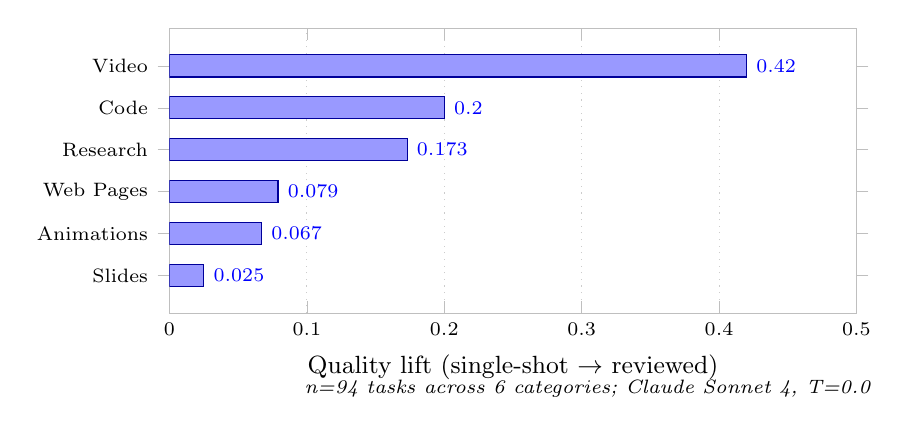
\begin{tikzpicture}
\begin{axis}[
  width=0.85\textwidth, height=5.2cm,
  xbar,
  xmin=0, xmax=0.5,
  bar width=8pt,
  enlarge y limits=0.18,
  symbolic y coords={Slides, Animations, Web Pages, Research, Code, Video},
  ytick=data,
  nodes near coords,
  nodes near coords align={horizontal},
  nodes near coords style={font=\scriptsize},
  every node near coord/.append style={/pgf/number format/.cd, fixed, precision=3},
  xlabel={Quality lift (single-shot $\to$ reviewed)},
  xtick={0, 0.1, 0.2, 0.3, 0.4, 0.5},
  major grid style={dotted, gray!40},
  xmajorgrids,
  axis line style={draw=gray!50},
  tick style={draw=gray!50},
  label style={font=\small},
  ticklabel style={font=\scriptsize},
]
\addplot+[draw=blue!60!black, fill=blue!40] coordinates {
  (0.025,Slides) (0.067,Animations) (0.079,Web Pages) (0.173,Research) (0.200,Code) (0.420,Video)
};
\end{axis}
\node[anchor=east, font=\scriptsize\itshape] at (current bounding box.south east)
  {n=94 tasks across 6 categories; Claude Sonnet 4, T=0.0};
\end{tikzpicture}
\caption{Phase 1 baseline: interaction-scaling lift orders by \emph{feedback actionability}. Execution feedback (Code: +0.20, Video: +0.42) is binary and machine-readable; factual verification (Research: +0.17) is specific but softer; visual feedback (Web: +0.08, Animations: +0.07, Slides: +0.03) is holistic and lossy to operationalize.}
\label{fig:actionability}
\end{figure}

\section{Phase 2 retrospective: why ``not distillable'' was wrong}
\label{app:phase2}

Earlier work in this project (Phase 2, text-only, Qwen3-8B, GRPO over a SFT'd model) reported that interaction scaling was \emph{not} distillable to 8B: the student matched the teacher's format but collapsed to 67\% identical-retries and gained 0pp pass@5 over base. Phase 5 retrospectively identifies the methodology error: the SFT labels stripped the teacher's reasoning, training the student on (input $\to$ critique + code) without scratch-space for diagnosis. With reasoning retained at the student's coherence horizon, identical-retry drops from 67\% to 9\% in-distribution.

\section{Pipeline implementation}
\label{app:pipeline}

The agentic pipeline consists of: a per-trajectory sandboxed workspace (\texttt{src/training/agent\_workspace.py}: tmpdir + 3 tools with path-traversal guards and a \texttt{python}$\to$\texttt{python3} shim); a teacher trace collector that calls the 235B model via OpenRouter with three tool schemas and a heavy system prompt walking the model through the verification loop (\texttt{src/training/collect\_agentic\_traces.py}); a Gemini multimodal judge that receives a per-step trace summary plus the final saved screenshot (\texttt{src/training/judge\_agentic\_traces.py}); a SFT prep step that collapses (\texttt{tool}-text + user-image\_url) workarounds back into a single \texttt{tool}-role message with image content (\texttt{src/training/prepare\_agentic\_sft.py}); and a student inference loop that parses \texttt{<tool\_call>\{json\}</tool\_call>} XML with a tolerant fallback for unescaped Python quotes inside JSON content fields (\texttt{src/training/run\_agent\_student.py}).

A critical bug in the SFT data loader, since fixed, was originally stripping the \texttt{tool\_calls} field from assistant messages during dataset reconstruction. The pre-fix model trained on text-only assistant turns followed by orphan tool responses, learning to emit \texttt{<|im\_end|>} immediately after introductory prose. After the fix, the unmasked label fraction rose from 16\% to 32\%, and the model emits valid \texttt{<tool\_call>} blocks at inference.

\section{Per-task pass@k breakdown for the markdown 8B student}
\label{app:per-task-md}

For comparison with \Cref{tab:per-task} on the agentic side, \Cref{tab:per-task-md} shows the per-task judge-keep outcome for the markdown V3+fc4k student across three independent samples.  Compared to the agentic v8 (which had 0 task overlap between greedy and $T{=}0.7$ seeds and 0/5 webpages at pass@3), the markdown student shows much higher base coverage (8/18 at pass@1 vs.\ 1/18) but \emph{also} substantial cross-seed diversity: pass@3 = 10/18 reflects 2 unique tasks added by sampling beyond the greedy-seed-1 set.

\begin{table}[ht]
\centering
\caption{Per-task judge-keep outcome for the markdown 8B student (V3+fc4k). $\checkmark$ = judge-kept; $\cdot$ = judge-rejected. Seed 1 is greedy ($T{=}0$); seeds 2--3 use $T{=}0.7$. The pass@3 column is the union.}
\label{tab:per-task-md}
\small
\begin{tabular}{llccccc}
\toprule
Category & Task & seed 1 ($T{=}0$) & seed 2 ($T{=}0.7$) & seed 3 ($T{=}0.7$) & pass@3 \\
\midrule
\multirow{5}{*}{webpages} & web\_002 & $\checkmark$ & $\cdot$ & $\cdot$ & $\checkmark$ \\
& web\_003 & $\checkmark$ & $\cdot$ & $\checkmark$ & $\checkmark$ \\
& web\_005 & $\cdot$ & $\cdot$ & $\cdot$ & $\cdot$ \\
& web\_008 & $\cdot$ & $\cdot$ & $\cdot$ & $\cdot$ \\
& web\_012 & $\cdot$ & $\cdot$ & $\cdot$ & $\cdot$ \\
\midrule
\multirow{8}{*}{slides} & slide\_001 & $\cdot$ & $\cdot$ & $\cdot$ & $\cdot$ \\
& slide\_006 & $\cdot$ & $\cdot$ & $\cdot$ & $\cdot$ \\
& slide\_007 & $\cdot$ & $\cdot$ & $\cdot$ & $\cdot$ \\
& slide\_008 & $\checkmark$ & $\cdot$ & $\cdot$ & $\checkmark$ \\
& slide\_010 & $\cdot$ & $\cdot$ & $\cdot$ & $\cdot$ \\
& slide\_014 & $\checkmark$ & $\checkmark$ & $\checkmark$ & $\checkmark$ \\
& slide\_018 & $\checkmark$ & $\checkmark$ & $\cdot$ & $\checkmark$ \\
& slide\_020 & $\cdot$ & $\checkmark$ & $\cdot$ & $\checkmark$ \\
\midrule
\multirow{5}{*}{code} & code\_h001 & $\checkmark$ & $\cdot$ & $\cdot$ & $\checkmark$ \\
& code\_h002 & $\checkmark$ & $\checkmark$ & $\cdot$ & $\checkmark$ \\
& code\_h003 & $\cdot$ & $\cdot$ & $\cdot$ & $\cdot$ \\
& code\_h004 & $\cdot$ & $\cdot$ & $\checkmark$ & $\checkmark$ \\
& code\_h005 & $\checkmark$ & $\checkmark$ & $\checkmark$ & $\checkmark$ \\
\midrule
\multicolumn{2}{r}{Total kept:} & 8/18 & 5/18 & 4/18 & \textbf{10/18 (56\%)} \\
\bottomrule
\end{tabular}
\end{table}

\section{Per-task pass@k breakdown for the agentic 8B student}
\label{app:per-task}

\Cref{tab:per-task} shows the per-task judge-keep outcome for the v8 (8B verbose, 51 SFT examples) configuration across three independent samples. Two observations are worth noting. \emph{First}, the seed-42 ($T{=}0$) and seed-43 ($T{=}0.7$) judge-kept sets have \emph{zero} task overlap --- different sampling regimes catch genuinely different tasks. \emph{Second}, all five webpage tasks fail across all three seeds; the structural visual floor is invariant to sampling. The pass@3 union of 4/18 thus comes entirely from code (3/5) and a single slide.

\begin{table}[ht]
\centering
\caption{Per-task judge-keep outcome for the agentic 8B student (v8, 51 SFT ex.). $\checkmark$ = judge-kept; $\cdot$ = judge-rejected. Seed 42 uses greedy decoding; seeds 43--44 use $T{=}0.7$. The pass@3 column is the union.}
\label{tab:per-task}
\small
\begin{tabular}{llccccc}
\toprule
Category & Task & seed 42 ($T{=}0$) & seed 43 ($T{=}0.7$) & seed 44 ($T{=}0.7$) & pass@3 \\
\midrule
\multirow{5}{*}{webpages} & web\_002 & $\cdot$ & $\cdot$ & $\cdot$ & $\cdot$ \\
& web\_003 & $\cdot$ & $\cdot$ & $\cdot$ & $\cdot$ \\
& web\_005 & $\cdot$ & $\cdot$ & $\cdot$ & $\cdot$ \\
& web\_008 & $\cdot$ & $\cdot$ & $\cdot$ & $\cdot$ \\
& web\_012 & $\cdot$ & $\cdot$ & $\cdot$ & $\cdot$ \\
\midrule
\multirow{8}{*}{slides} & slide\_001 & $\cdot$ & $\cdot$ & $\cdot$ & $\cdot$ \\
& slide\_006 & $\cdot$ & $\cdot$ & $\cdot$ & $\cdot$ \\
& slide\_007 & $\cdot$ & $\cdot$ & $\cdot$ & $\cdot$ \\
& slide\_008 & $\cdot$ & $\cdot$ & $\cdot$ & $\cdot$ \\
& slide\_010 & $\cdot$ & $\cdot$ & $\cdot$ & $\cdot$ \\
& slide\_014 & $\cdot$ & $\cdot$ & $\cdot$ & $\cdot$ \\
& slide\_018 & $\cdot$ & $\checkmark$ & $\cdot$ & $\checkmark$ \\
& slide\_020 & $\cdot$ & $\cdot$ & $\cdot$ & $\cdot$ \\
\midrule
\multirow{5}{*}{code} & code\_h001 & $\checkmark$ & $\cdot$ & $\cdot$ & $\checkmark$ \\
& code\_h002 & $\cdot$ & $\cdot$ & $\cdot$ & $\cdot$ \\
& code\_h003 & $\cdot$ & $\cdot$ & $\cdot$ & $\cdot$ \\
& code\_h004 & $\cdot$ & $\checkmark$ & $\cdot$ & $\checkmark$ \\
& code\_h005 & $\cdot$ & $\checkmark$ & $\cdot$ & $\checkmark$ \\
\midrule
\multicolumn{2}{r}{Total kept:} & 1/18 & 3/18 & 0/18 & \textbf{4/18 (22\%)} \\
\bottomrule
\end{tabular}
\end{table}

\section{Inter-judge agreement (Gemini vs.\ Claude)}
\label{app:interjudge}

We re-judged two trace sets with Claude Sonnet 4.5 (anthropic/claude-sonnet-4-5 via OpenRouter) using the identical judge prompt and the same final-screenshot evidence. Per-trace agreement is shown in \Cref{tab:interjudge}.

\begin{table}[ht]
\centering
\caption{Inter-judge agreement between Gemini~3 Flash Preview (primary) and Claude Sonnet 4.5 (sensitivity). Cohen's $\kappa$ over the 36 traces is +0.55 (moderate agreement). Claude is consistently stricter on visual artifacts: it rejects 5 of 8 visual tasks that Gemini accepts in the V3+fc4k markdown set. The directional gap (markdown $\gg$ agentic) is preserved under either judge.}
\label{tab:interjudge}
\small
\begin{tabular}{lcccc}
\toprule
Set & Gemini & Claude & \% agree & Cohen's $\kappa$ \\
\midrule
V3+fc4k seed1 (markdown 8B) & 8/18 & 3/18 & 72\% & +0.40 \\
v8 seed42 (agentic 8B) & 1/18 & 1/18 & 100\% & +1.00 \\
\midrule
\textbf{Combined (n=36)} & \textbf{9/36} & \textbf{4/36} & \textbf{86\%} & \textbf{+0.55} \\
\bottomrule
\end{tabular}
\end{table}

The five tasks where the judges disagree are all visual: Gemini accepts \texttt{slide\_008}, \texttt{slide\_014}, \texttt{slide\_018}, \texttt{web\_002}, and \texttt{web\_003} as judge-keep on the markdown student; Claude rejects each by inspecting the rendered screenshot and finding specific layout or styling violations the agent overlooked. We interpret this as Claude having a higher bar on ``does the artifact actually meet the spec'' rather than as Gemini being noisy --- both judges produce internally consistent ratings on the same trace twice.

\section{Hyperparameters and SFT details}
\label{app:hyperparams}

All SFT runs use AdamW with linear warmup-then-decay learning rate (peak $2{\times}10^{-4}$), per-device batch size 1, gradient accumulation 8, 3 epochs, gradient checkpointing (non-reentrant), bf16 (or NF4-double-quant for QLoRA). LoRA targets language-layer attention projections (\texttt{q,k,v,o\_proj}) and MLP projections (\texttt{gate,up,down\_proj}); vision tower is frozen. For 4-bit base (32B), \texttt{bitsandbytes} \texttt{nf4} with \texttt{bnb\_4bit\_use\_double\_quant=True} and \texttt{bnb\_4bit\_compute\_dtype=bf16}. For 8-bit base (30B-A3B), we skip \texttt{prepare\_model\_for\_kbit\_training} entirely (its fp32 promotion of all non-quantized parameters doubles memory in MoE) and instead manually enable gradient checkpointing and \texttt{enable\_input\_require\_grads}. Inference for both formats uses greedy decoding ($T{=}0$) for single-shot evaluation and $T{=}0.7$ with $\mathrm{rep\_penalty}{=}1.0$ for sampling.

\end{document}
